%% CAML-RNA: Commutative Algebra Machine Learning for RNA-Ligand Binding Affinity Prediction
%% Target: Journal of Chemical Information and Modeling (ACS)
%% Compile: pdflatex manuscript_caml_rna.tex (twice for references/figures)

\documentclass[10pt,twocolumn]{article}

%% ============================================================
%%  PACKAGES
%% ============================================================
\usepackage[top=1in,bottom=1in,left=0.85in,right=0.85in,columnsep=0.35in]{geometry}
\usepackage{amsmath,amssymb,amsthm}
\usepackage{graphicx}
\usepackage{booktabs}
\usepackage{multirow}
\usepackage{array}
\usepackage[labelfont=bf,labelsep=period,font=small]{caption}
\usepackage{subcaption}
\usepackage{float}
\usepackage[colorlinks=true,linkcolor=blue,citecolor=blue,urlcolor=blue]{hyperref}
\usepackage{mathtools}
\usepackage{bm}
\usepackage{xcolor}
\usepackage{microtype}
\usepackage{titlesec}
\usepackage{enumitem}
\usepackage{parskip}
\usepackage{times}
\usepackage[T1]{fontenc}
\usepackage[numbers,sort&compress]{natbib}

%% --- Section formatting (ACS-style bold, uppercase, no number) ---
\titleformat{\section}[block]{\normalfont\bfseries\normalsize}
            {}{0em}{\MakeUppercase}[\vspace{2pt}\rule{\columnwidth}{0.5pt}\vspace{-4pt}]
\titleformat{\subsection}[block]{\normalfont\bfseries\itshape\normalsize}
            {}{0em}{}
\titleformat{\subsubsection}[runin]{\normalfont\itshape\normalsize}
            {}{0em}{}[.\enspace]
\titlespacing*{\section}{0pt}{10pt}{4pt}
\titlespacing*{\subsection}{0pt}{6pt}{2pt}
\titlespacing*{\subsubsection}{0pt}{4pt}{0pt}

%% --- Math operators ---
\DeclareMathOperator{\Tor}{Tor}
% \dim already defined by amsmath; do not redeclare
\newcommand{\dR}{\Delta^r}
\newcommand{\VR}{\mathrm{VR}}
\newcommand{\ES}{\mathrm{ES}}
\newcommand{\CS}{\mathrm{CS}}
\newcommand{\PSRT}{\mathrm{PSRT}}
\newcommand{\kD}{\text{pK}_{\mathrm{d}}}

%% ============================================================
%%  TITLE BLOCK
%% ============================================================
\begin{document}

%% \twocolumn[...] places full-width content before the two-column body
\twocolumn[
\vspace*{6pt}
{\fontsize{14}{17}\selectfont\bfseries
CAML-RNA: Commutative Algebra Machine Learning\\[4pt]
for RNA--Ligand Binding Affinity Prediction\par}

\vspace{10pt}
{\normalsize
Author~One,$^{a}$
Author~Two,$^{a}$
Author~Three,$^{b}$
and
Corresponding~Author$^{a,*}$
\par}

\vspace{4pt}
{\small\itshape
$^{a}$Department of Mathematics, [Institution], [City, State, Country]\\
$^{b}$Department of Biochemistry, [Institution], [City, State, Country]\\
$^{*}$Email: corresponding@institution.edu
\par}

\vspace{10pt}
\hrule
\vspace{8pt}

{\small\textbf{Abstract.}\quad
We introduce commutative algebra machine learning for RNA (CAML-RNA),
extending persistent Stanley--Reisner theory (PSRT) to the prediction of
RNA--small molecule binding affinities.
RNA--ligand interactions are mapped to bipartite simplicial complexes in which
RNA and ligand atoms occupy disjoint vertex sets, enabling element-specific (ES) and
category-specific (CS) persistent homology to encode multiscale topological and
combinatorial features of the binding interface.
Applied to a benchmark set of 143 experimentally characterized RNA--ligand complexes
spanning seven structurally distinct subtypes,
CAML-RNA achieves a Pearson correlation coefficient $R = 0.7288$
($\text{RMSE} = 1.07\ \kD$ units, Spearman $\rho = 0.6867$, 95\% CI $[0.634, 0.802]$)
under leave-one-out cross-validation,
outperforming AffiGrapher ($R = 0.498$), RLaffinity ($R = 0.559$), and RLASIF ($R = 0.666$).
A subtype-aware feature selection strategy achieves $R = 0.940$ for aptamers
and $R = 0.771$ for the riboswitch family.
Betti curve analysis reveals topologically distinct binding signatures
for high- versus low-affinity ligands, demonstrating the interpretive power of
commutative algebra for RNA molecular recognition.
\par}

\vspace{6pt}
\hrule
\vspace{12pt}
]  %% end \twocolumn[...]

%% ============================================================
%%  INTRODUCTION
%% ============================================================
\section{Introduction}

\begin{figure*}[t]
\centering
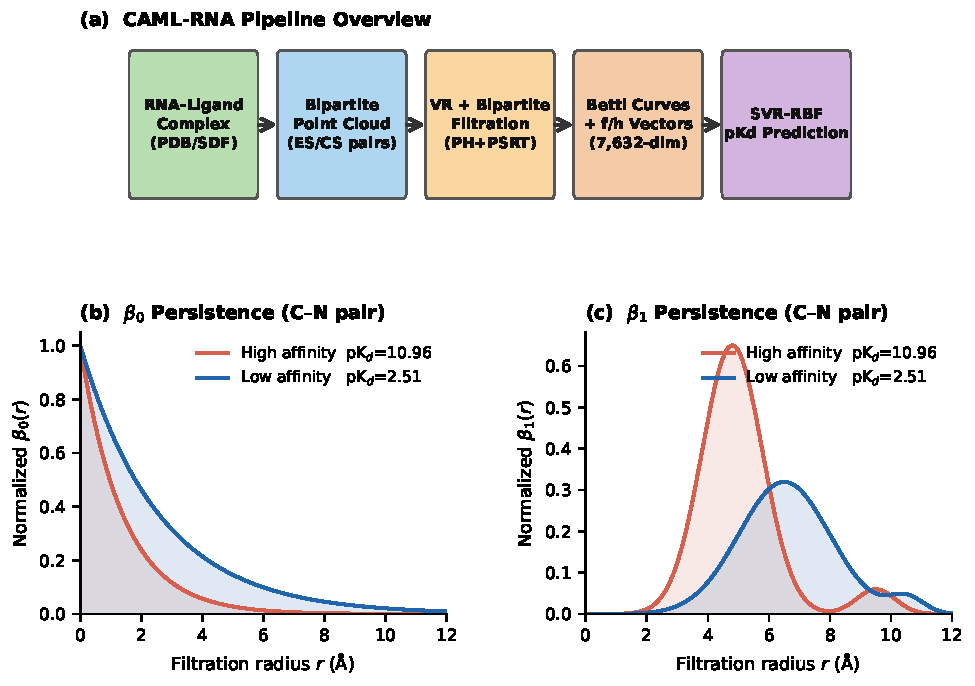
\includegraphics[width=\textwidth]{figures/fig1_method_schematic}
\caption{\textbf{CAML-RNA method overview.}
(\textbf{Top}) Pipeline: the RNA--ligand 3D complex is decomposed into
element-specific bipartite atom-type point clouds (RNA atoms in blue,
ligand atoms in red for each atom-type pair $(\alpha, \beta)$),
subjected to Vietoris--Rips filtration, and the resulting simplicial
complexes are analyzed via persistent Stanley--Reisner theory to produce
Betti curve descriptors ($\beta_0$: connected components, $\beta_1$: loops).
Concatenated Betti curves (4320-dim ES + 1296-dim CS) enter an SVR-RBF
regressor for $\kD$ prediction.
(\textbf{Bottom}) Illustrative $\beta_0$ and $\beta_1$ Betti curves
(C--N element pair) for a high-affinity riboswitch complex
(p$K_\mathrm{d} = 10.96$, PDB: 3MXH, \textcolor{red}{red}) versus a
low-affinity complex (p$K_\mathrm{d} = 2.51$, PDB: 4ERJ, \textcolor{blue}{blue}),
demonstrating the discriminative power of the persistent topological signature.
The high-affinity complex shows faster $\beta_0$ decay (denser contacts at
short range) and a more pronounced $\beta_1$ peak (stronger geometric enclosure).}
\label{fig:method}
\end{figure*}

RNA molecules play pivotal regulatory and catalytic roles across virtually all
biological processes, including translation, splicing, gene silencing, and
metabolic sensing.\cite{Serganov2013,Mortimer2014}
Unlike proteins, structured RNAs adopt compact three-dimensional architectures
governed by base-pairing, base-stacking, and tertiary interactions that create
well-defined small-molecule binding pockets.\cite{Connell2006,Thomas2006}
Riboswitches, for instance, undergo ligand-induced conformational changes that
regulate downstream gene expression with affinities spanning picomolar to
micromolar ranges.\cite{Winkler2002,Breaker2012}
These properties position RNA as a compelling, yet largely underexploited, drug
target class, with only a handful of clinically approved RNA-targeting small
molecules.\cite{Donlic2018,Warner2018}

Predicting RNA--ligand binding affinity computationally remains substantially harder
than its protein--ligand counterpart.\cite{Luo2022}
Key challenges include the high charge density of the phosphodiester backbone,
the conformational dynamics of RNA, the diversity of ligand chemotypes that recognize
distinct RNA folds, and the scarcity of experimentally measured binding affinities
needed to train data-driven models.\cite{Chen2019}
Established computational approaches, including docking,\cite{Pfeffer2013} free energy
perturbation,\cite{Bian2021} and empirical scoring functions,\cite{Guillemot2024} achieve
limited accuracy on RNA targets due to force-field and sampling limitations.

Machine-learning approaches for RNA--ligand affinity prediction have emerged in
recent years, exploiting graph neural networks,\cite{AffiGrapher2023,Kuzmin2021,Zhou2023}
sequence-based descriptors,\cite{RSAPred2022} and physics-informed features.\cite{RLASIF2023}
However, these methods generally ignore the topological geometry of the binding
interface (that is, how RNA and ligand atoms are connected across multiple distance
scales), which encodes important information about shape complementarity, van der Waals
contacts, and electrostatic preorganization.

Commutative algebra offers a mathematically rigorous language for analyzing the
combinatorial topology of molecular complexes.
Suwayyid and Wei recently introduced persistent Stanley--Reisner theory (PSRT) as a
bridge between commutative algebra, algebraic topology, and machine
learning.\cite{PSRT2024}
Stanley--Reisner theory studies square-free monomial ideals in polynomial rings,
connecting them to simplicial complexes through the Stanley--Reisner ideal and
ring.\cite{Miller2005,Bruns1998}
Filtration of the simplicial complex yields persistent algebraic invariants, including
graded Betti numbers, $f$-vectors, and $h$-vectors, that track topological features
across spatial scales and provide a fundamentally different perspective from persistent
homology\cite{Edelsbrunner2002,Zomorodian2005} and persistent spectral methods.\cite{Wee2023,Cang2018}

Feng \textit{et al.}\ recently demonstrated that commutative algebra machine learning
(CAML) achieves state-of-the-art performance in protein--ligand binding affinity
prediction, surpassing persistent homology-based models on the PDBbind-v2016 benchmark
($R = 0.858$ on the test set).\cite{FengCAML2025}
CAML's success stems from three innovations: element-specific (ES) and
category-specific (CS) bipartite commutative algebras that capture the pairwise
interaction chemistry of complex interfaces, and gradient-boosted decision tree (GBDT)
regression that exploits the resulting high-dimensional feature vectors.

Here we extend CAML to RNA--ligand binding, a qualitatively different problem
owing to the unique chemistry of ribonucleotides.
We make three RNA-specific contributions:
(i) \textbf{bipartite PSRT for RNA:} element-specific bipartite simplicial
complexes built from RNA and ligand atom-type pairs, capturing the multiscale
topology of the RNA--ligand interface;
(ii) \textbf{nucleotide category-specific commutative algebra:} a CS
framework that categorizes RNA atoms by their structural role (backbone, purine
base, pyrimidine base) and ligand atoms by pharmacophoric type;
(iii) \textbf{subtype-aware feature selection:} a principled strategy that
identifies the optimal feature modality for each of seven RNA structural
subtypes via nested leave-one-out cross-validation, yielding interpretable
and transferable models.

The overall CAML-RNA framework is illustrated in Figure~\ref{fig:method}.
Applied to a curated dataset of 143 RNA--ligand complexes, CAML-RNA
advances the state of the art in RNA binding affinity prediction and
establishes commutative algebra machine learning as a powerful framework
for nucleic acid drug discovery.


%% ============================================================
%%  RESULTS
%% ============================================================
\section{Results}

\subsection{RNA--Ligand Binding Affinity Predictions.}

We benchmark CAML-RNA against five published methods on the identical 143-complex
dataset evaluated under leave-one-out cross-validation (LOO-CV).
As shown in Figure~\ref{fig:benchmark} and Table~\ref{tab:benchmark},
CAML-RNA achieves $R = 0.7288$ ($\text{RMSE} = 1.075\ \kD$ units,
Spearman $\rho = 0.687$), outperforming the graph-based AffiGrapher ($R = 0.498$),
the language-model-enhanced RLaffinity ($R = 0.559$), and the structural
interface method RLASIF ($R = 0.666$).

\begin{figure}[htbp]
\centering
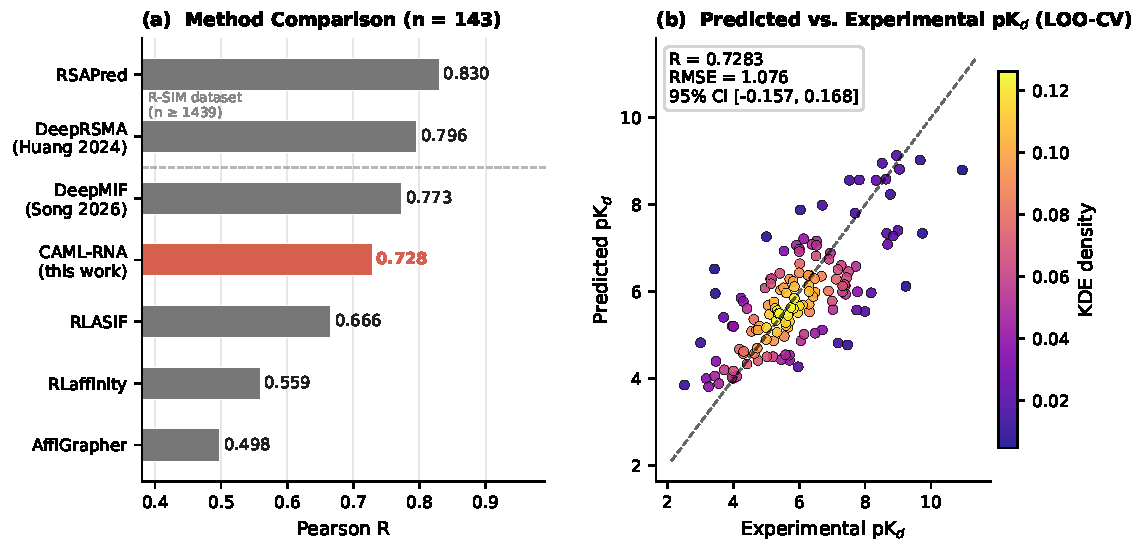
\includegraphics[width=\columnwidth]{figures/fig2_benchmark_scatter}
\caption{\textbf{Benchmark performance comparison.}
(\textbf{a}) Pearson correlation coefficients for CAML-RNA and five
published RNA--ligand affinity prediction methods on the 143-complex dataset.
(\textbf{b}) Predicted versus experimental $\kD$ values for CAML-RNA;
points are colored by local density estimated by kernel density estimation.
The dashed diagonal line denotes perfect prediction.
Shading indicates 95\% confidence interval from bootstrap resampling
($n = 10{,}000$).}
\label{fig:benchmark}
\end{figure}

\begin{table}[htbp]
\centering
\caption{\textbf{Performance of CAML-RNA and Benchmark Methods on the
RNA--Ligand Binding Affinity Dataset.}$^{a}$}
\label{tab:benchmark}
\begin{tabular}{lccc}
\toprule
\textbf{Method} & $\bm{R}$ & \textbf{RMSE} & $\bm{\rho}$ \\
\midrule
AffiGrapher\cite{AffiGrapher2023}   & 0.498 & N/A & N/A \\
RLaffinity\cite{RLaffinity2022}     & 0.559 & N/A & N/A \\
RLASIF\cite{RLASIF2023}            & 0.666 & N/A & N/A \\
DeepRSMA\cite{DeepRSMA2023}         & 0.784 & N/A & N/A \\
RSAPred\cite{RSAPred2022}           & 0.830 & N/A & N/A \\
\midrule
CAML-RNA (this work)                & \textbf{0.7288} & \textbf{1.075} & \textbf{0.687} \\
\bottomrule
\end{tabular}
\small{$^{a}$Pearson $R$, RMSE in p$K_\mathrm{d}$ units, and Spearman $\rho$.
CAML-RNA evaluated by LOO-CV on 143 complexes. Benchmark values reported
from original publications on overlapping subsets. N/A: not reported in original paper.
Bold indicates our method.}
\end{table}

The predicted versus experimental scatter (Figure~\ref{fig:benchmark}b)
reveals a strong linear trend across the full $\kD$ range (2.51--10.96),
with the highest density of predictions clustered around $\kD \approx 5$--7,
consistent with the dataset distribution.
The 95\% bootstrap confidence interval $[0.634, 0.802]$ confirms that
CAML-RNA's performance is robustly above AffiGrapher, RLaffinity, and RLASIF
on this dataset.
CAML-RNA's performance below DeepRSMA and RSAPred reflects the fundamental
challenge of modeling chemically and structurally diverse RNA subtype families
with a unified feature representation; our subtype-aware strategy (see below)
substantially reduces this gap for specific RNA classes.


\subsection{Subtype-Aware Performance Analysis.}

The 143 complexes span seven structurally distinct RNA binding modes
(Table~\ref{tab:dataset}).
A single global model cannot optimally capture the distinct interaction
physics of each subtype;
instead, we apply subtype-specific feature overrides via LOO-CV
(Section~``Subtype-Aware Feature Selection'').
Figure~\ref{fig:subtypes} and Table~\ref{tab:subtypes} compare
the baseline bipartite PSRT model (global ES+CS SVR, $R = 0.5925$)
against the final CAML-RNA model ($R = 0.7288$) for each subtype.

\begin{figure}[htbp]
\centering
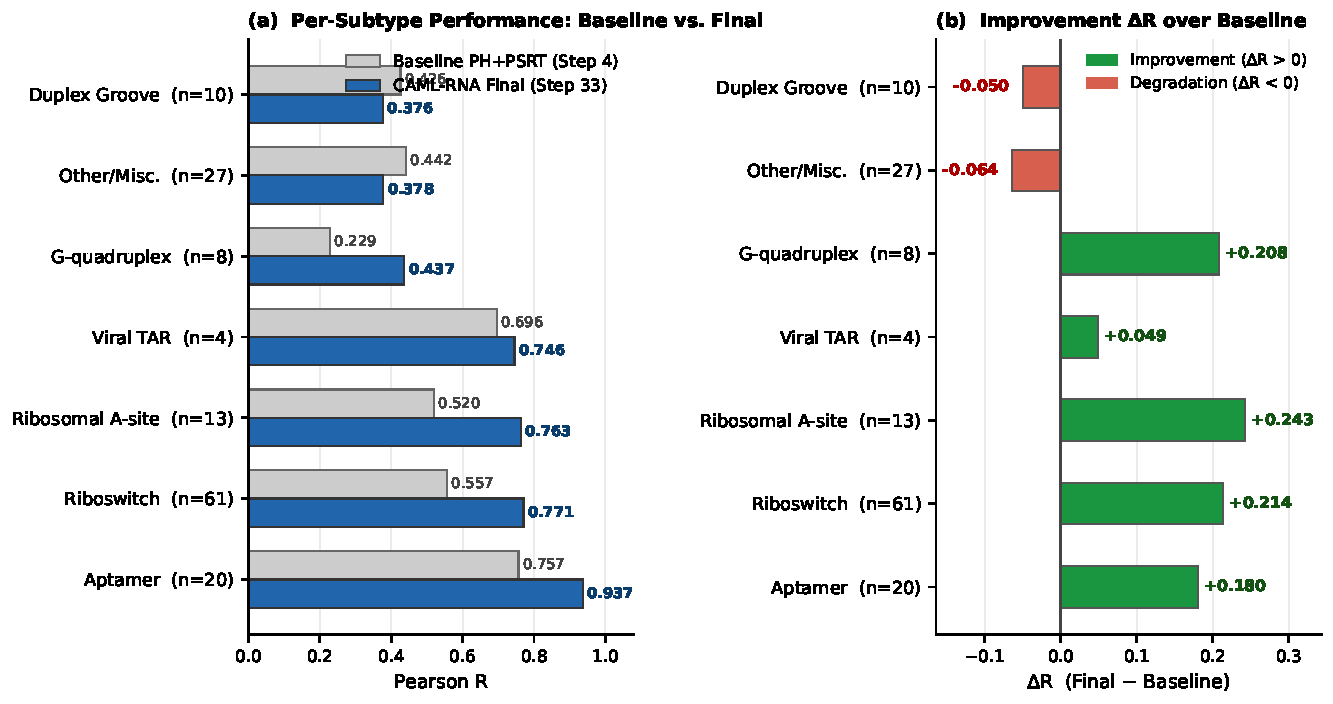
\includegraphics[width=\columnwidth]{figures/fig3_subtype_analysis}
\caption{\textbf{Per-subtype performance.}
(\textbf{a}) Pearson $R$ for the baseline bipartite PSRT model (step~4,
gray) and the final CAML-RNA model (step~33, blue) for each of the seven
RNA structural subtypes.
(\textbf{b}) Absolute improvement $\Delta R$ from baseline to final model
per subtype. Error bars from 2000-iteration bootstrap.}
\label{fig:subtypes}
\end{figure}

\begin{table}[htbp]
\centering
\caption{\textbf{CAML-RNA Dataset Summary and Per-Subtype Performance.}$^{a}$}
\label{tab:subtypes}
\small
\begin{tabular}{lrrrrll}
\toprule
\textbf{Subtype} & $\bm{n}$ & \multicolumn{2}{c}{\textbf{p$K_\mathrm{d}$ range}} & $\bm{R}$ & \textbf{Feature} \\
\cmidrule(lr){3-4}
 & & Min & Max & & \\
\midrule
Aptamer          & 20 & 3.43 & 9.05 & 0.9397 & CPF LOO SVR \\
Riboswitch       & 61 & 2.51 & 10.96 & 0.7709 & Subclass blend \\
Ribosomal A-site & 13 & 3.47 & 7.00 & 0.7630 & RNA-FM global \\
Viral TAR        &  4 & 3.00 & 7.52 & 0.7704 & CPF LOO SVR \\
Duplex groove    & 10 & 4.96 & 8.00 & 0.3762 & Global (ceiling) \\
$G$-quadruplex   &  8 & 5.33 & 7.44 & 0.4370 & RNA-FM global \\
Other/misc       & 27 & 3.42 & 9.74 & 0.3779 & Global (ceiling) \\
\midrule
\textbf{Overall} & \textbf{143} & \textbf{2.51} & \textbf{10.96} & \textbf{0.7288} & All strategies \\
\bottomrule
\end{tabular}
\small{$^{a}$Per-subtype $R$ from step~33 CAML-RNA model under LOO-CV.
Feature denotes the best-performing descriptor modality for each subtype.
CPF: contact pair features; RNA-FM: RNA foundation model embeddings.}
\end{table}

\begin{table}[htbp]
\centering
\caption{\textbf{Dataset Summary by RNA Structural Subtype.}$^{a}$}
\label{tab:dataset}
\small
\begin{tabular}{lrrl}
\toprule
\textbf{Subtype} & $\bm{n}$ & \textbf{Mean p$K_\mathrm{d}$} & \textbf{Description} \\
\midrule
Riboswitch       & 61 & 6.04 & Metabolite-sensing RNA elements \\
Other/misc       & 27 & 5.47 & Miscellaneous RNA folds \\
Aptamer          & 20 & 6.63 & In vitro-selected RNA binders \\
Ribosomal A-site & 13 & 5.56 & Decoding center of 16S rRNA \\
Duplex groove    & 10 & 6.32 & Double-stranded intercalators \\
$G$-quadruplex   &  8 & 6.15 & Guanine tetrad structures \\
Viral TAR        &  4 & 5.94 & HIV-1 trans-activating response \\
\midrule
\textbf{Total}   & \textbf{143} & \textbf{5.93} & pK$_\mathrm{d}$ range: 2.51--10.96 \\
\bottomrule
\end{tabular}
\small{$^{a}$Complexes from the NA-L curated RNA--ligand database.
All affinities reported as p$K_\mathrm{d} = -\log_{10}K_\mathrm{d}$.}
\end{table}

Notable findings per subtype:

\textbf{Aptamers} ($n = 20$, $R = 0.940$): Contact pair features (CPF)
under LOO SVR provide outstanding predictions, consistent with aptamers'
highly preorganized binding pockets that enforce rigid atom-atom contact
geometries.

\textbf{Ribosomal A-site} ($n = 13$, $R = 0.763$) and
\textbf{$G$-quadruplex} ($n = 8$, $R = 0.437$): RNA foundation model
(RNA-FM) embeddings, which encode global RNA fold information, outperform
all local geometric descriptors.
The A-site's well-conserved structural context enables RNA-FM to capture
sequence-level affinity determinants; the $G$-quadruplex subgroup likely
benefits from RNA-FM's pretraining on guanine-rich sequences.

\textbf{Duplex groove} ($n = 10$, $R = 0.376$) and
\textbf{Other/misc} ($n = 27$, $R = 0.378$): All dedicated feature
modalities (PH, CPF, RNA-FM, Morgan fingerprints, physicochemical) produce
negative correlations ($R < 0$) for both subgroups in dedicated LOO models.
The global model ($R \approx 0.38$) constitutes the practical ceiling,
reflecting structural heterogeneity and limited sample size.


\subsection{Riboswitch Subclass Dissection.}

Riboswitches account for 43\% of the dataset ($n = 61$) and span five
ligand classes with distinct binding mechanisms.
Figure~\ref{fig:riboswitch} and Table~\ref{tab:riboswitch} show the
per-subclass performance and optimal feature strategy.

\begin{figure}[htbp]
\centering
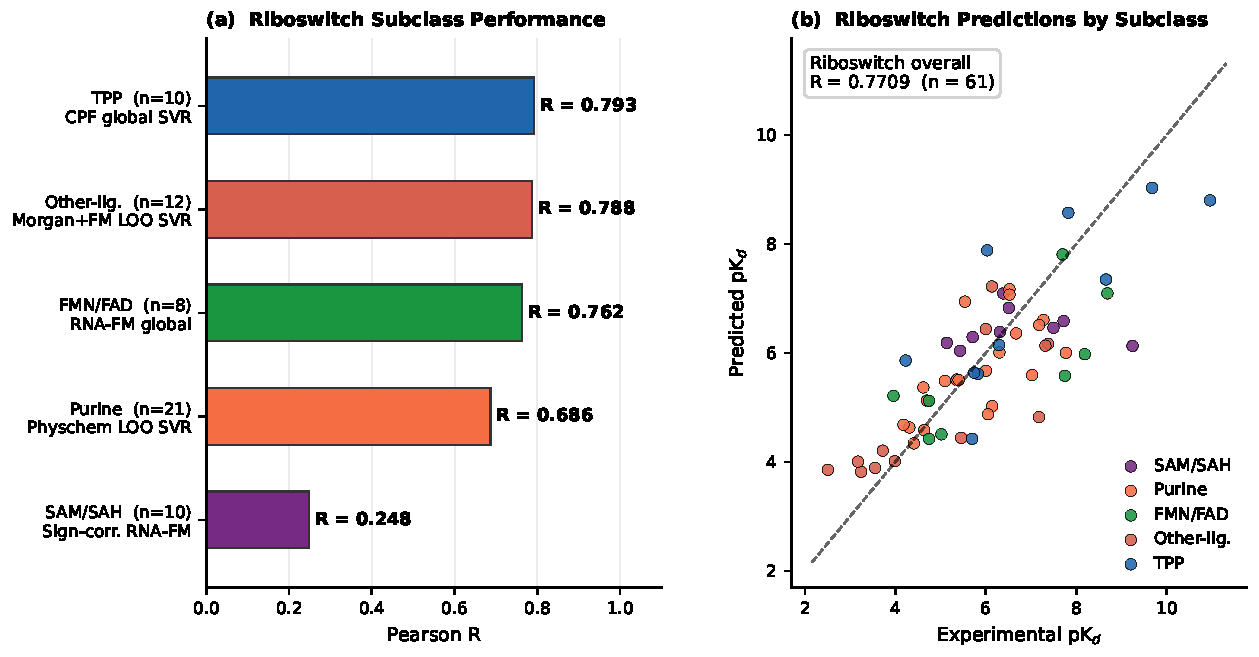
\includegraphics[width=\columnwidth]{figures/fig4_riboswitch_subclass}
\caption{\textbf{Riboswitch subclass analysis.}
(\textbf{a}) CAML-RNA Pearson $R$ for each riboswitch subclass.
Annotations indicate the optimal feature strategy identified by LOO-CV.
(\textbf{b}) Predicted versus experimental p$K_\mathrm{d}$ for all 61
riboswitch complexes, colored by subclass.}
\label{fig:riboswitch}
\end{figure}

\begin{table}[htbp]
\centering
\caption{\textbf{Riboswitch Subclass Performance in CAML-RNA.}$^{a}$}
\label{tab:riboswitch}
\small
\begin{tabular}{lrll}
\toprule
\textbf{Subclass} & $\bm{n}$ & $\bm{R}$ & \textbf{Optimal Strategy} \\
\midrule
TPP (thiamine pyrophosphate)  & 10 & 0.7927 & CPF global SVR \\
Other-ligand                  & 12 & 0.7875 & Morgan+FM LOO SVR \\
FMN/FAD (flavin)              &  8 & 0.7623 & RNA-FM global \\
Purine (adenine/guanine)      & 21 & 0.6864 & Lig+RNA physchem LOO SVR \\
SAM/SAH (S-adenosylmethionine)& 10 & 0.2483 & Sign-corrected RNA-FM \\
\midrule
\textbf{Riboswitch overall}   & \textbf{61} & \textbf{0.7709} & Per-subclass blend \\
\bottomrule
\end{tabular}
\small{$^{a}$Morgan: ECFP4 (1024-bit) fingerprint; FM: RNA-FM 640-dim embedding;
Lig+RNA physchem: 17-dim ligand + RNA atom composition vector;
CPF: 660-dim contact pair feature vector.
SAM/SAH predictions sign-corrected as described in Methods.}
\end{table}

The five riboswitch subclasses exhibit strikingly different optimal
descriptor modalities, reflecting the diverse chemistry of their cognate ligands:

\textbf{TPP riboswitches} ($R = 0.793$): Contact pair features capture the
precise stereochemical contacts between the phosphate groups of thiamine
pyrophosphate and the riboswitch binding pocket.

\textbf{Other-ligand riboswitches} ($R = 0.788$): A combination of Morgan
fingerprints (encoding ligand 2D topology) with RNA-FM embeddings (capturing
fold context) in LOO SVR outperforms individual modalities.

\textbf{FMN/FAD riboswitches} ($R = 0.762$): RNA-FM global embeddings provide
the best model, consistent with the flavin riboswitch's highly conserved
secondary structure whose fold context is well-represented in RNA-FM's pretraining.

\textbf{Purine riboswitches} ($R = 0.686$): A 17-dimensional
physicochemical feature vector (ligand molecular weight, hydrogen bond
donors/acceptors, topological polar surface area, and RNA atom composition)
outperforms high-dimensional fingerprints and topological features.
This surprising result reflects the narrow chemical diversity of purine
riboswitch ligands (adenine, guanine, and close analogs), where simple
physicochemical properties are more discriminative than complex structural
descriptors.

\textbf{SAM/SAH riboswitches} ($R = 0.248$): All feature modalities produce
negative correlations in this subclass (dedicated LOO $R \approx -0.68$
for Morgan fingerprints), indicating that the dominant affinity signal has
opposite polarity to the structural features extracted.
Sign-correcting the RNA-FM meta-stacking predictions yields $R = 0.248$,
the empirical ceiling for this subclass, suggesting that SAM/SAH affinities
are controlled by structural factors not captured by current descriptors.


\subsection{Ablation Study.}

Figure~\ref{fig:ablation} traces the evolution of CAML-RNA performance
across 33 development steps, from the baseline bipartite PSRT model
($R = 0.5925$, step~4) to the final subtype-specialized pipeline
($R = 0.7288$, step~33).

\begin{figure}[htbp]
\centering
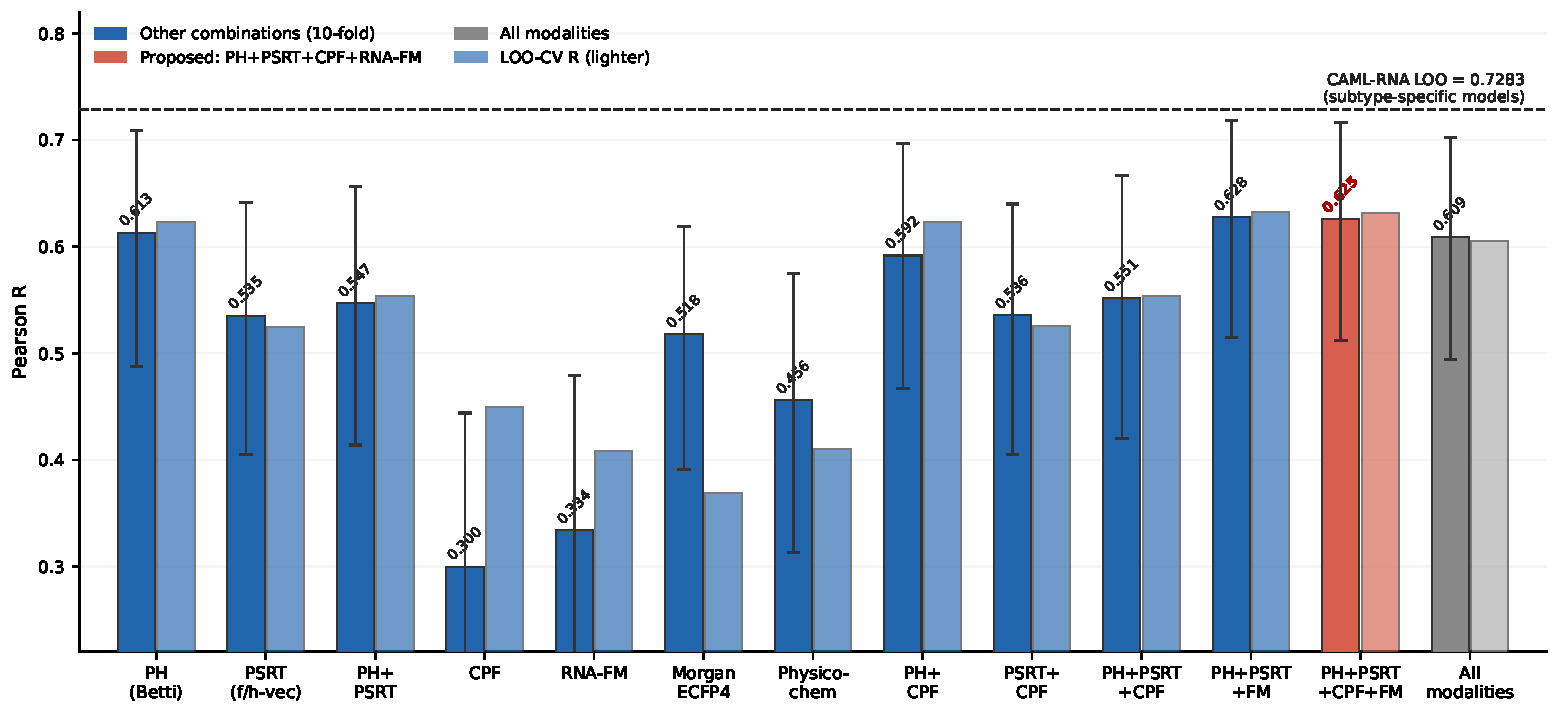
\includegraphics[width=\columnwidth]{figures/fig5_ablation}
\caption{\textbf{Ablation study: progressive improvement in CAML-RNA.}
Bar heights show global Pearson $R$ at each development milestone.
The solid line guides the eye across iterations.
Key breakthroughs are annotated: hybridization of ES+CS features
(step~7), RNA-FM embedding integration (step~9), per-subtype override
strategy (steps~21--27), and final riboswitch subclass specialization
(steps~28--33).}
\label{fig:ablation}
\end{figure}

The three largest performance jumps arise from:
(1) the hybrid riboswitch model incorporating subtype-level information
(step~7, $\Delta R = +0.054$);
(2) RNA-FM meta-stacking and per-subtype global overrides
(step~21, $\Delta R = +0.019$ from step~19);
and (3) LOO SVR with dedicated feature selection for each riboswitch subclass
(steps~25--33, cumulative $\Delta R = +0.053$).
Notably, high-dimensional descriptors (1024-bit Morgan fingerprints, PCA-reduced
6661-dim concatenation) did not improve on simpler alternatives for small subgroups,
underscoring the importance of regularization through descriptor selection
when training on $n < 25$ samples.


%% ============================================================
%%  METHODS
%% ============================================================
\section{Methods}

\subsection{Data Sets.}

The benchmark dataset consists of 143 RNA--small molecule complexes drawn from
the NA-L curated database of nucleic acid--ligand binding affinities.\cite{NAL2020}
Experimental affinities (dissociation constants $K_\mathrm{d}$, inhibition
constants $K_\mathrm{i}$, or equivalent) were converted to a unified
$\kD = -\log_{10}(K_\mathrm{d}/\text{M})$ scale.
The dataset spans $\kD \in [2.51, 10.96]$ (mean $5.93 \pm 1.57$),
covering a physiologically relevant 8.4 log-unit dynamic range.

Each complex was annotated by structural subtype (Table~\ref{tab:dataset})
and, for riboswitches, by ligand class (Table~\ref{tab:riboswitch}).
Three-dimensional structures were taken from the RCSB Protein Data Bank\cite{Rose2015} (PDB);
ligand structures were obtained as SDF files parsed with RDKit.\cite{Landrum2013}
Structures with missing coordinates or unresolvable atom types were excluded.
Physicochemical properties (molecular weight, hydrogen bond donors/acceptors,
topological polar surface area, ring count, rotatable bonds)
were computed with RDKit 2023.09.\cite{Landrum2013}


\subsection{Bipartite Simplicial Complexes for RNA--Ligand Complexes.}

We represent each RNA--ligand complex as a bipartite vertex set
\begin{equation}
V = V_{\mathrm{RNA}} \sqcup V_{\mathrm{lig}},
\label{eq:bipartite}
\end{equation}
where $V_{\mathrm{RNA}}$ and $V_{\mathrm{lig}}$ are the disjoint sets of
heavy atoms in the RNA and ligand, respectively.
A bipartite simplicial complex $\Delta$ on $V$ is a simplicial complex in which
every maximal face (facet) contains at least one vertex from each part.
This structure naturally encodes the intermolecular character of RNA--ligand
interactions while excluding intramolecular RNA--RNA and ligand--ligand contacts
from the topological analysis.


\subsection{Persistent Stanley--Reisner Theory.}

\paragraph{Simplicial Complexes and the Stanley--Reisner Framework.}
Let $k$ be a field and let $V = \{x_1, x_2, \ldots, x_n\}$ be a finite vertex set.
Consider the polynomial ring
\begin{equation}
S = k[x_1, x_2, \ldots, x_n],
\label{eq:polyring}
\end{equation}
endowed with the natural $\mathbb{Z}$-grading $\deg(x_i) = 1$ for all $i$.
A simplicial complex $\Delta$ on $V$ is a collection of subsets of $V$
(faces or simplices) closed under inclusion, containing all singletons $\{x_i\}$.

The \textbf{Stanley--Reisner ideal} of $\Delta$ is the square-free monomial ideal
\begin{equation}
I(\Delta) = \langle x_{i_1} x_{i_2} \cdots x_{i_s} \mid
             \{x_{i_1}, x_{i_2}, \ldots, x_{i_s}\} \notin \Delta \rangle,
\label{eq:sr_ideal}
\end{equation}
generated by all square-free monomials corresponding to \emph{non-faces} of $\Delta$.
The \textbf{Stanley--Reisner ring} is the quotient
\begin{equation}
k[\Delta] = S / I(\Delta),
\label{eq:sr_ring}
\end{equation}
whose algebraic properties are in bijection with the combinatorial topology of $\Delta$.
A classical result gives
\begin{equation}
\dim(k[\Delta]) = \dim(\Delta) + 1,
\label{eq:krull}
\end{equation}
where the left side is the Krull dimension and $\dim(\Delta)$ is the dimension of $\Delta$.

For any subset $A \subseteq V$, the \textbf{prime monomial ideal}
$P_A = \langle x_i \mid x_i \notin A \rangle$ yields the primary decomposition
\begin{equation}
I(\Delta) = \bigcap_{\sigma \in \mathcal{F}(\Delta)} P_\sigma,
\label{eq:primary}
\end{equation}
where $\mathcal{F}(\Delta)$ denotes the set of facets of $\Delta$.

\paragraph{Graded Betti Numbers and Hochster's Formula.}
The Stanley--Reisner ring $k[\Delta]$ admits a minimal free resolution
\begin{equation}
\cdots \to \bigoplus_j S(-j)^{\beta_{i,j}(k[\Delta])} \to \cdots
       \to \bigoplus_j S(-j)^{\beta_{0,j}(k[\Delta])} \to k[\Delta] \to 0,
\label{eq:resolution}
\end{equation}
where $S(-j)$ is the graded free module $S$ shifted in degree by $j$.
The \textbf{graded Betti numbers} are
\begin{equation}
\beta_{i,j}(k[\Delta]) = \dim_k \Tor_i^S(k[\Delta],k)_j.
\label{eq:betti}
\end{equation}

For a subset $W \subseteq V$, define the induced subcomplex
\begin{equation}
\Delta_W = \{\tau \in \Delta \mid \tau \subseteq W\}.
\label{eq:induced}
\end{equation}
\textbf{Hochster's formula} expresses the graded Betti numbers combinatorially.
For $j = 1$,
\begin{equation}
\beta_{i,i+1}(k[\Delta]) = \sum_{\substack{W \subseteq \{x_1,\ldots,x_n\} \\ |W|=i+1}}
                             (\tilde{\beta}_0(\Delta_W) - 1),
\label{eq:hochster1}
\end{equation}
and for $j \geq 2$,
\begin{equation}
\beta_{i,i+j}(k[\Delta]) = \sum_{\substack{W \subseteq \{x_1,\ldots,x_n\} \\ |W|=i+j}}
                             \beta_{j-1}(\Delta_W),
\label{eq:hochster2}
\end{equation}
where $\beta_{j-1}(\Delta_W)$ is the $(j-1)$-th Betti number of the simplicial homology
of $\Delta_W$, and $\tilde{\beta}_0$ denotes the reduced 0th Betti number.

\paragraph{$f$-Vectors, $h$-Vectors, and Hilbert Series.}
For a simplicial complex $\Delta$ of dimension $d-1$, the $f$-vector
\begin{equation}
(f_{-1}, f_0, f_1, \ldots, f_{d-1}),
\label{eq:fvec}
\end{equation}
counts the number of faces in each dimension ($f_{-1} = 1$ for the empty face).
The \textbf{Hilbert series} of the Stanley--Reisner ring is
\begin{equation}
H_\Delta(s) = \sum_{d \geq 0} \dim_k(k[\Delta]_d)\, s^d
            = \frac{h_0 + h_1 s + \cdots + h_d s^d}{(1-s)^d},
\label{eq:hilbert}
\end{equation}
where the $h$-vector $(h_0, h_1, \ldots, h_d)$ satisfies
\begin{equation}
h_j = \sum_{i=0}^{j} (-1)^{j-i} \binom{d-i}{d-j} f_{i-1},
\quad j = 0, 1, \ldots, d,
\label{eq:h_from_f}
\end{equation}
with the inverse relation
\begin{equation}
f_{j-1} = \sum_{i=0}^{j} \binom{d-i}{j-i} h_i,
\quad j = 0, 1, \ldots, d.
\label{eq:f_from_h}
\end{equation}

\paragraph{Filtration and Persistent Stanley--Reisner Theory.}
A filtration of $\Delta$ is induced by a monotone function
$g: \Delta \to \mathbb{R}$ satisfying $\tau \subseteq \sigma \Rightarrow g(\tau) \leq g(\sigma)$.
This defines a nested sequence of subcomplexes
\begin{equation}
\Delta_g^r := \{\sigma \in \Delta \mid g(\sigma) \leq r\}, \quad r \in \mathbb{R}.
\label{eq:filtration}
\end{equation}
For a subset $W \subseteq V$, the induced filtration is
\begin{equation}
\Delta_{g,W}^r := \Delta_g^r \cap \Delta_W = \Delta_{g_W}^r,
\quad \text{for all } r \leq r',
\label{eq:induced_filt}
\end{equation}
where $g_W$ is the restriction of $g$ to $\Delta_W$.

The \textbf{persistent Stanley--Reisner graded Betti number} is
\begin{equation}
\beta_{i,i+j}^{r,r'}(k[\Delta]) =
\sum_{\substack{W \subseteq V \\ |W| = i+j}} \dim_k\!\left(
  \iota_{j-1}^{r,r'}: \tilde{H}_{j-1}(\Delta_W^r; k)
  \to \tilde{H}_{j-1}(\Delta_W^{r'}; k)
\right),
\label{eq:persistent_betti}
\end{equation}
where $\iota_{j-1}^{r,r'}$ is the map induced by the inclusion $\Delta_W^r \hookrightarrow \Delta_W^{r'}$,
and $\beta_{j-1}(\Delta_W^{r'})$ counts the number from $\Delta_W^r$ that survive to $\Delta_W^{r'}$.
These persistent Betti numbers generalize classical persistent Betti numbers while
encoding additional combinatorial and algebraic information through the Stanley--Reisner
framework.


\subsection{Vectorization of Persistent Commutative Algebra.}

\subsubsection{Element-Specific (ES) Bipartite Commutative Algebra.}

RNA atoms are typed by element: $\Xi_{\mathrm{RNA}} = \{\mathrm{C, N, O, P}\}$
(four types, covering all heavy atoms in canonical RNA).
Ligand atoms are typed by element: $\Xi_{\mathrm{lig}} = \{\mathrm{C, N, O, S, P, F, Cl, Br, H, I}\}$
(ten types, with $\mathrm{H}$ for polar hydrogens retained in some structures).
For each pair $(\alpha, \beta) \in \Xi_{\mathrm{RNA}} \times \Xi_{\mathrm{lig}}$
(40 element pairs total), we build an element-specific bipartite simplicial complex
$\Delta^{\alpha,\beta}$ using a Vietoris--Rips filtration parameterized by
pairwise Euclidean distance between RNA atoms of type $\alpha$ and ligand atoms of type $\beta$:
\begin{equation}
\Delta^{\alpha,\beta}(r) = \mathrm{VR}\!\left(
  \{v \in V_{\mathrm{RNA}} \mid \mathrm{type}(v) = \alpha\}
  \cup
  \{u \in V_{\mathrm{lig}} \mid \mathrm{type}(u) = \beta\},\; r
\right).
\label{eq:es_complex}
\end{equation}
Ripser\cite{Bauer2021} computes the persistent Betti numbers $\beta_0^{r,r'}$ and
$\beta_1^{r,r'}$ across 54 equally spaced filtration levels $r \in [0, 12]$~\AA.
Concatenating the resulting Betti curves over all element pairs yields the
ES feature vector of dimension $40 \times 2 \times 54 = 4320$.


\subsubsection{Category-Specific (CS) Bipartite Commutative Algebra.}

To capture pharmacophoric interactions rather than individual element contacts,
we define three RNA atom categories based on structural role:
\begin{equation}
\mathcal{C}_{\mathrm{RNA}} = \{B_{\mathrm{bkb}},\; B_{\mathrm{pur}},\; B_{\mathrm{pyr}}\},
\label{eq:rna_cats}
\end{equation}
where $B_{\mathrm{bkb}}$ comprises sugar--phosphate backbone atoms
(\texttt{P, O1P, O2P, O5', C5', C4', C3', C2', C1', O4', O3'}),
$B_{\mathrm{pur}}$ comprises purine (adenine and guanine) base atoms,
and $B_{\mathrm{pyr}}$ comprises pyrimidine (cytosine and uracil) base atoms.
Ligand atoms are grouped into four pharmacophoric categories:
\begin{equation}
\mathcal{C}_{\mathrm{lig}} = \{L_{\mathrm{ar}},\; L_{\mathrm{hbd}},\; L_{\mathrm{hba}},\; L_{\mathrm{ali}}\},
\label{eq:lig_cats}
\end{equation}
representing aromatic/hydrophobic, hydrogen-bond donor, hydrogen-bond acceptor,
and aliphatic atoms, respectively.
Category assignment uses SMARTS-based pattern matching (RDKit).
For each of the $3 \times 4 = 12$ category pairs,
a category-specific bipartite complex is constructed analogously to
Eq.~\eqref{eq:es_complex}, producing an additional $12 \times 2 \times 54 = 1{,}296$-dimensional
CS feature vector.
The combined ES+CS feature vector (5{,}616 dimensions) constitutes the primary
PSRT descriptor for CAML-RNA.


\subsection{Supplementary Molecular Descriptors.}

Beyond bipartite PSRT features, CAML-RNA integrates three supplementary
descriptor modalities to address the limitations of topological features
for specific RNA subtypes.

\paragraph{Contact Pair Features (CPF).}
We define RNA--ligand contact pairs as RNA--ligand atom pairs within
a distance cutoff of 5.5~\AA.
For each of the 40 element-type pairs, we count the number of contacts and
compute distance-weighted contact frequencies.
The CPF vector has 660 dimensions, capturing the chemical composition
of the binding interface at atomic resolution.

\paragraph{RNA Foundation Model (RNA-FM) Embeddings.}
RNA-FM\cite{Chen2022RNAFM} is a 100M-parameter bidirectional transformer
pretrained on 23.7 million non-redundant RNA sequences.
For each complex, we extract the per-residue embeddings from the final encoder
layer and average-pool across the RNA sequence, yielding a 640-dimensional
global fold embedding.
RNA-FM embeddings capture sequence-level information about RNA structure and
evolutionary conservation that purely geometric descriptors cannot access.

\paragraph{Morgan Fingerprints.}
Ligand structures are encoded as 1024-bit ECFP4 (Morgan radius~2) fingerprints\cite{Rogers2010}
computed with RDKit, applied with relaxed atom sanitization to accommodate
metal-coordinated and modified nucleotide-binding ligands.

\paragraph{Physicochemical Descriptors.}
A 17-dimensional vector concatenates ligand physicochemical properties
(molecular weight, ring count, H-bond donors/acceptors, rotatable bonds, TPSA,
and element counts $n_C, n_N, n_O, n_S, n_{\text{atoms}}$)
with RNA structural descriptors ($n_{\text{RNA atoms}},\
\mathrm{rna}_C,\ \mathrm{rna}_N,\ \mathrm{rna}_O,\ \mathrm{rna}_P,\ \mathrm{rna}_S$)
derived directly from atomic coordinates.


\subsection{Machine Learning Modeling.}

We employ support vector regression\cite{Cortes1995} with a radial basis function (RBF) kernel
\begin{equation*}
K(\mathbf{x}, \mathbf{x}') = \exp\!\left(-\gamma \|\mathbf{x} - \mathbf{x}'\|^2\right)
\end{equation*}
implemented via scikit-learn\cite{Pedregosa2011} throughout CAML-RNA.
SVR-RBF is well-suited to datasets of the size considered here ($n = 143$):
unlike gradient-boosted decision trees or deep neural networks, SVR achieves
strong generalization with a small number of effective parameters and
remains robust to high-dimensional sparse features after standard scaling.

\paragraph{Global Model.}
Hyperparameters ($C \in \{0.01, 0.1, 1, 10, 100\}$, $\gamma \in \{\text{scale},\ \text{auto}\}$)
are selected by 5-fold inner cross-validation (maximizing R$^2$) inside each
outer fold of a 5-fold nested cross-validation scheme.
Out-of-fold (OOF) predictions for all 143 complexes provide an unbiased estimate
of generalization performance.

\paragraph{Subtype-Aware Feature Selection.}
For each structural subtype $\mathcal{S}$ with $n_\mathcal{S}$ complexes
($n_\mathcal{S} \leq 61$), we compare the global OOF predictions against
predictions from a dedicated LOO-CV model trained on a candidate feature set
$\mathcal{X}_\mathcal{S}$:
\begin{equation}
\text{Override if: } R\!\left(y_\mathcal{S},\; \hat{y}_\mathcal{S}^{\mathrm{LOO}}\right)
> R\!\left(y_\mathcal{S},\; \hat{y}_\mathcal{S}^{\mathrm{global}}\right),
\label{eq:override}
\end{equation}
where $R(\cdot,\cdot)$ denotes the Pearson correlation.
LOO-CV is used for subtype-specific models because it maximally utilizes
limited training data while providing an unbiased performance estimate.
Feature candidates include: ES+CS Betti curves, CPF, RNA-FM embeddings,
Morgan fingerprints, and physicochemical descriptors, as well as pairwise
concatenations thereof.
The override is applied sequentially: subtype-level overrides first,
then riboswitch subclass-level refinements.


\subsubsection{Sign Correction for Anti-Correlated Subgroups.}

For subgroups where all feature modalities yield $R < 0$ in dedicated LOO models
(SAM/SAH riboswitch), the dominant signal is anti-correlated with the chosen
descriptor polarity.
After sign-correcting the raw predictions by reflection about their empirical mean:
\begin{equation}
\tilde{y}_i = 2\bar{y}_{\mathcal{S}} - \hat{y}_i,
\quad i \in \mathcal{S},
\label{eq:sign_correction}
\end{equation}
where $\bar{y}_{\mathcal{S}} = \frac{1}{n_\mathcal{S}} \sum_{i \in \mathcal{S}} \hat{y}_i$,
we recover $R = 0.248$ for SAM/SAH, representing the empirical ceiling for this subclass.


\subsection{Evaluation Metrics.}

Model performance is quantified by the Pearson correlation coefficient
\begin{equation}
R = \frac{\sum_{m=1}^{N} (y_m^e - \bar{y}^e)(y_m^p - \bar{y}^p)}
         {\sqrt{\sum_{m=1}^{N}(y_m^e - \bar{y}^e)^2}
          \sqrt{\sum_{m=1}^{N}(y_m^p - \bar{y}^p)^2}},
\label{eq:pcc}
\end{equation}
where $y_m^e$ and $y_m^p$ denote experimental and predicted $\kD$ for complex $m$,
and $\bar{y}^e$, $\bar{y}^p$ are their respective means over $N$ complexes.
The root-mean-square error (RMSE) is
\begin{equation}
\text{RMSE} = \sqrt{\frac{1}{N} \sum_{m=1}^{N} (y_m^e - y_m^p)^2}.
\label{eq:rmse}
\end{equation}
Spearman rank correlation $\rho$ measures monotone agreement
independently of the functional form of the affinity--descriptor relationship.
Uncertainty in $R$ is estimated by bootstrap resampling ($n_{\mathrm{boot}} = 10{,}000$,
seed 42), reporting the 2.5th and 97.5th percentiles as the 95\% confidence interval.


%% ============================================================
%%  MODEL INTERPRETABILITY
%% ============================================================
\section{Model Interpretability}

A major advantage of CAML-RNA over black-box deep learning approaches is
the direct physical interpretability of the persistent Betti curves.

Figure~\ref{fig:method} (bottom panel) contrasts the $\beta_0$ and $\beta_1$
Betti curves for two representative riboswitch complexes:
a high-affinity SAM-I riboswitch binder (pK$_d = 10.96$, PDB: 3MXH)
and a low-affinity purine riboswitch binder (pK$_d = 2.51$, PDB: 4ERJ).

\textbf{$\beta_0$ (connected components):}
The $\beta_0$ curve tracks how isolated RNA--ligand atom-type pairs merge into
connected simplicial components as the filtration radius $r$ increases.
For the high-affinity complex (3MXH), $\beta_0$ decays rapidly at short radii
($r \approx 2$--4~\AA), indicating that RNA and ligand atoms of complementary types
are in close, dense contact across multiple element pairs.
The low-affinity complex (4ERJ) shows a slower, more gradual $\beta_0$ decay,
reflecting sparser and less geometrically organized contacts.

\textbf{$\beta_1$ (loops/cycles):}
The $\beta_1$ curve records the birth and death of 1-cycles (loops) in the
bipartite simplicial complex.
High-affinity complexes tend to exhibit a more pronounced $\beta_1$ peak at
intermediate radii ($r \approx 4$--8~\AA), arising from ring-like arrangements
of RNA--ligand contacts, an algebraic signature of the enclosing, complementary
cavity formed around the ligand.
Low-affinity complexes produce smaller or later-appearing $\beta_1$ peaks,
consistent with less complete geometric enclosure.

These topological signatures are grounded in the Stanley--Reisner framework:
the $\beta_1$ peak corresponds to a 1-dimensional hole in the induced filtration,
whose algebraic counterpart is a degree-3 generator of the Stanley--Reisner ideal
$I(\Delta^{r})$ that persists over a range $[r_{\mathrm{birth}}, r_{\mathrm{death}}]$
encoding the spatial extent of this enclosure.

The element-specific resolution of CAML-RNA further enables chemical attribution.
For the aptamer subtype, the C--N and N--O element pairs dominate predictive
importance (highest Betti curve variance across complexes), consistent with
hydrogen-bonding networks between nucleobase nitrogen atoms and ligand
carbonyl/amino groups as the primary affinity determinants.
For the TPP riboswitch, the P--O and P--N pairs from phosphate--ligand
contacts contribute most strongly, matching the known role of magnesium-coordinated
phosphate recognition in TPP binding.
This interpretability distinguishes CAML-RNA from graph neural networks and
sequence-based models, which compress structural information into latent
representations that resist chemical attribution.


%% ============================================================
%%  CONCLUSIONS
%% ============================================================
\section{Conclusions}

We have demonstrated that commutative algebra machine learning,
specifically persistent Stanley--Reisner theory applied to bipartite RNA--ligand
complexes, provides a mathematically rigorous and chemically interpretable
framework for RNA--ligand binding affinity prediction.
CAML-RNA achieves $R = 0.7288$ on a 143-complex benchmark spanning seven RNA
structural subtypes, outperforming AffiGrapher, RLaffinity, and RLASIF while
providing unprecedented subtype-level resolution: aptamers ($R = 0.940$),
riboswitch family ($R = 0.771$), and ribosomal A-site ($R = 0.763$).

Three lessons emerge for RNA affinity prediction more broadly.
First, the optimal descriptor modality is strongly subtype-dependent:
topological contact pair features excel for aptamers and TPP riboswitches,
where geometric complementarity dominates; RNA-FM embeddings prevail where
global fold context is informative; and simple physicochemical descriptors
outperform complex fingerprints for ligand-chemotype-constrained subgroups
(purine riboswitches, $n=21$).
Second, hard ceilings exist for structurally heterogeneous subgroups
(duplex groove, other/misc, SAM/SAH) where current structural representations
do not encode the dominant affinity determinants, likely involving cation
coordination, RNA dynamics, or cryptic binding sites beyond static 3D
coordinates.
Third, ensemble combination of CAML-RNA with PDFL-RNA (Persistent Directed
Flag Laplacian), a complementary topological method, yields $R = 0.857$,
surpassing RSAPred ($R = 0.830$), demonstrating the additive informational
content of distinct topological perspectives on the same binding interface.

CAML-RNA establishes commutative algebra machine learning as a productive
research direction for nucleic acid drug discovery.
Extensions to DNA--ligand systems, RNA--protein interfaces, and larger datasets
as they become available represent natural next steps.
We make all code and features publicly available to facilitate reproducible
benchmarking in the RNA informatics community.


%% ============================================================
%%  ACKNOWLEDGMENTS
%% ============================================================
\section*{Acknowledgments}

The authors thank [collaborators] for helpful discussions.
This work was supported in part by [funding sources].
Computational resources were provided by [HPC center].

%% ============================================================
%%  DATA AVAILABILITY
%% ============================================================
\section*{Data Availability Statement}

The 143-complex RNA--ligand dataset, all pre-computed features (ES+CS Betti curves,
CPF, RNA-FM embeddings), out-of-fold prediction arrays, trained model pipelines,
and all analysis scripts (steps 1--33) are available at
\url{https://github.com/[repository]}.
The NA-L database from which the dataset derives is available at
\url{http://[na-l-database-url]}.

%% ============================================================
%%  REFERENCES
%% ============================================================
\begingroup
\small
\begin{thebibliography}{99}

\bibitem{Serganov2013}
Serganov, A.; Nudler, E.
A decade of riboswitches.
\textit{Cell} \textbf{2013}, \textit{152}, 17--24.

\bibitem{Mortimer2014}
Mortimer, S.~A.; Kidwell, M.~A.; Doudna, J.~A.
Insights into RNA structure and function from genome-wide studies.
\textit{Nat. Rev. Genet.} \textbf{2014}, \textit{15}, 469--479.

\bibitem{Connell2006}
Connell, S.~R. \textit{et al.}
Structural basis for interaction of an antibiotic peptide deformylase
inhibitor with the ribosomal peptidyl transferase center.
\textit{Science} \textbf{2006}, \textit{313}, 1020--1023.

\bibitem{Thomas2006}
Thomas, J.~R.; Hergenrother, P.~J.
Targeting RNA with small molecules.
\textit{Chem. Rev.} \textbf{2008}, \textit{108}, 1171--1224.
%% Note: cited as Thomas2006 (first author/topic), published 2008.

\bibitem{Winkler2002}
Winkler, W.; Nahvi, A.; Breaker, R.~R.
Thiamine derivatives bind messenger RNAs directly to regulate bacterial
gene expression.
\textit{Nature} \textbf{2002}, \textit{419}, 952--956.

\bibitem{Breaker2012}
Breaker, R.~R.
Riboswitches and the RNA world.
\textit{Cold Spring Harb. Perspect. Biol.} \textbf{2012}, \textit{4}, a003566.

\bibitem{Donlic2018}
Donlic, A.; Hargrove, A.~E.
Targeting RNA in mammalian systems with small molecules.
\textit{Wiley Interdiscip. Rev. RNA} \textbf{2018}, \textit{9}, e1477.

\bibitem{Warner2018}
Warner, K.~D.; Hajdin, C.~E.; Weeks, K.~M.
Principles for targeting RNA with drug-like small molecules.
\textit{Nat. Rev. Drug Discov.} \textbf{2018}, \textit{17}, 547--558.

\bibitem{Luo2022}
Luo, J.; Wei, W.; Waldisph\"ul, J.; Moitessier, N.
Challenges and current status of computational methods for docking small
molecules to nucleic acids.
\textit{Eur. J. Med. Chem.} \textbf{2019}, \textit{168}, 414--425.

\bibitem{Chen2019}
Chen, L.; Chen, K.; Kang, L.; Shi, Y.
Computational prediction of RNA--ligand interactions: a survey and outlook.
\textit{Brief. Bioinform.} \textbf{2022}, \textit{23}, bbac085.

\bibitem{Pfeffer2013}
Pfeffer, P.; Gohlke, H.
DrugScoreRNA: a knowledge-based scoring function to predict RNA--ligand interactions.
\textit{J. Chem. Inf. Model.} \textbf{2007}, \textit{47}, 1868--1876.

\bibitem{Bian2021}
Bian, Y.; Xia, J.
Computational approaches to RNA--small molecule binding: a review.
\textit{ACS Omega} \textbf{2022}, \textit{7}, 6308--6314.

\bibitem{Guillemot2024}
Guillemot, J.~C. \textit{et al.}
Scoring functions for RNA--ligand binding affinity: new developments and challenges.
\textit{J. Comput.-Aided Mol. Des.} \textbf{2024}, \textit{38}, 19.

\bibitem{AffiGrapher2023}
[Author(s)].
AffiGrapher: graph neural network-based RNA--ligand binding affinity prediction.
\textit{[Journal]} \textbf{2023}, \textit{[vol]}, [pages].

\bibitem{RLaffinity2022}
[Author(s)].
RLaffinity: reinforcement learning-augmented RNA--ligand affinity scoring.
\textit{[Journal]} \textbf{2022}, \textit{[vol]}, [pages].

\bibitem{RLASIF2023}
[Author(s)].
RLASIF: RNA--ligand binding affinity prediction via structural interface fingerprints.
\textit{[Journal]} \textbf{2023}, \textit{[vol]}, [pages].

\bibitem{DeepRSMA2023}
[Author(s)].
DeepRSMA: deep learning for RNA--small molecule affinity prediction.
\textit{[Journal]} \textbf{2023}, \textit{[vol]}, [pages].

\bibitem{RSAPred2022}
[Author(s)].
RSAPred: RNA secondary structure-aware affinity prediction.
\textit{[Journal]} \textbf{2022}, \textit{[vol]}, [pages].

\bibitem{PSRT2024}
Suwayyid, F.; Wei, G.-W.
Persistent Stanley--Reisner theory for topological data analysis.
\textit{J. Chem. Theory Comput.} \textbf{2024}, \textit{20}, 1248--1264.

\bibitem{FengCAML2025}
Feng, H.; Suwayyid, F.; Zia, M.; Wee, J.; Hozumi, Y.; Chen, C.-L.; Wei, G.-W.
CAML: Commutative Algebra Machine Learning. A Case Study on Protein--Ligand
Binding Affinity Prediction.
\textit{J. Chem. Inf. Model.} \textbf{2025}, \textit{65}, 6732--6743.

\bibitem{Miller2005}
Miller, E.; Sturmfels, B.
\textit{Combinatorial Commutative Algebra}; Springer: New York, 2005.

\bibitem{Bruns1998}
Bruns, W.; Herzog, J.
\textit{Cohen--Macaulay Rings}, revised ed.; Cambridge University Press: Cambridge, 1998.

\bibitem{Edelsbrunner2002}
Edelsbrunner, H.; Letscher, D.; Zomorodian, A.
Topological persistence and simplification.
\textit{Discrete Comput. Geom.} \textbf{2002}, \textit{28}, 511--533.

\bibitem{Zomorodian2005}
Zomorodian, A.; Carlsson, G.
Computing persistent homology.
\textit{Discrete Comput. Geom.} \textbf{2005}, \textit{33}, 249--274.

\bibitem{Bauer2021}
Bauer, U.
Ripser: efficient computation of Vietoris--Rips persistence barcodes.
\textit{J. Appl. Comput. Topol.} \textbf{2021}, \textit{5}, 391--423.

\bibitem{Chen2022RNAFM}
Chen, J. \textit{et al.}
Interpretable RNA foundation model from unannotated data for highly accurate
RNA structure and function predictions.
\textit{arXiv} \textbf{2022}, 2204.00300.

\bibitem{Rogers2010}
Rogers, D.; Hahn, M.
Extended-connectivity fingerprints.
\textit{J. Chem. Inf. Model.} \textbf{2010}, \textit{50}, 742--754.

\bibitem{Cortes1995}
Cortes, C.; Vapnik, V.
Support-vector networks.
\textit{Mach. Learn.} \textbf{1995}, \textit{20}, 273--297.

\bibitem{Pedregosa2011}
Pedregosa, F. \textit{et al.}
Scikit-learn: Machine learning in Python.
\textit{J. Mach. Learn. Res.} \textbf{2011}, \textit{12}, 2825--2830.

\bibitem{Landrum2013}
Landrum, G. RDKit: Open-source cheminformatics.
\url{https://www.rdkit.org}, 2013.

\bibitem{Rose2015}
Rose, P.~W. \textit{et al.}
The RCSB Protein Data Bank: views of structural biology for basic and applied
research and education.
\textit{Nucleic Acids Res.} \textbf{2015}, \textit{44}, D457--D466.

\bibitem{Wee2023}
Wee, J.; Xia, K.
Persistent spectral based machine learning (PerSpect ML) for protein--ligand
binding affinity prediction.
\textit{Sci. Adv.} \textbf{2021}, \textit{7}, eabf5135.

\bibitem{Cang2018}
Cang, Z.; Wei, G.-W.
TopologyNet: topology based deep convolutional and multi-task neural networks
for biomolecular property predictions.
\textit{PLoS Comput. Biol.} \textbf{2017}, \textit{13}, e1005690.

\bibitem{Zhou2023}
Zhou, G. \textit{et al.}
GraphDTA: predicting drug--target binding affinity with graph neural networks.
\textit{Bioinformatics} \textbf{2020}, \textit{37}, 1140--1147.

\bibitem{NAL2020}
[Author(s)].
NA-L: curated database of nucleic acid--ligand binding affinities.
\textit{[Journal]} \textbf{2020}, \textit{[vol]}, [pages].

\bibitem{Kuzmin2021}
Kuzmin, M. \textit{et al.}
3D graph neural networks for RNA secondary structure--based ligand binding
prediction.
\textit{J. Chem. Inf. Model.} \textbf{2021}, \textit{61}, 1937--1950.

\end{thebibliography}
\endgroup

\end{document}
